\documentclass[../main.tex]{subfiles}

\begin{document}
\chapter{Drivers of Antarctic Land Ice}
\label{chap:land_ice}
In chapter \ref{chap:temp_and_ice}, we found that temperature is significant for our understanding of the trends in Antarctic \gls{sic} over the last 40 years. However we found that the relationship between temperature and land ice is not as strong. To understand this we will have to do some more calculations.

We want to consider a range of variables which could be impacting land ice in Antarctica. We will include temperature again for completeness. Wind speed is linked to atmospheric circulations which move clouds and thermal energy around the continent. Cloud cover has also been linked to behaviours in the land ice. \textcolor{red}{add appropriate citations here}. 

\section{Time-frame of datasets used in this chapter}
For this chapter we use a number of datasets, which each have data available for different time frames. Because of the limitations in table \ref{tab:landicedata} we will restrict our time-frame to 2014 - 2017.
% Please add the following required packages to your document preamble:
% \usepackage{booktabs}
\begin{table}[H]
\begin{tabular}{@{}lll@{}}
\toprule
Data                                     & Start Date   & End Date \\ \midrule
ECMWF ERA5 Reanalysis                    & January 1981 & Present  \\
GRACE \gls{LILWET}                       & August 2002  & 2017  \\
ARGO product \textcolor{red}{check this} & January 2004 & Present  \\ \bottomrule
\end{tabular}
\caption{Different data sources used in this chapter.}
\label{tab:landicedata}
\end{table}

\section{Land ice trends and variability}
Before we start investigating what drives the changes in antarctic land ice, let's look again at the trends and behaviours seen in land ice specifically. We are interested in if the variables have impact on sea ice, however we have determined that sea ice trends and variability are largely driven by temperature, and so will not plot the trends and variability in sea ice again here.

The first plot to consider is the mean state of \gls{lilwet} (see Figure \ref{fig:lilwet_mean}).
 \begin{figure}[!hbt]
     \centering
     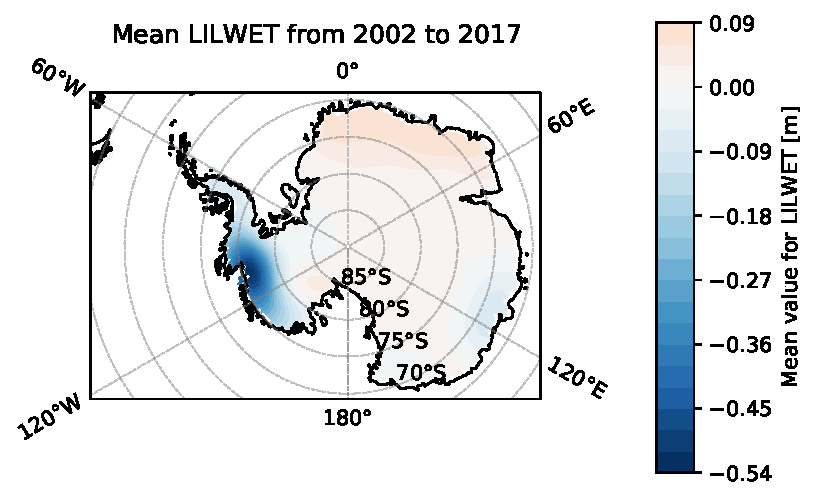
\includegraphics{images/2021w5/chapter7/hres/mean_spatial_LIC}
     \caption{Mean value of \gls{lilwet} from 2002 to 2017.}
     \label{fig:lilwet_mean}
 \end{figure}
 Looking at figure \ref{fig:lilwet_mean} we observe small values over most of the continent (maximum of 9 cm) whereas we have negative values of \gls{lilwet} over west Antarctica. The negative values are consequential of the way the data was measured (see Chapter \ref{chap:data} for more detail). The \gls{lilwet} data is anomalous from a baseline \textcolor{red}{check what this baseline is}. This indicates that the \gls{wais} is a good place to focus our attention. For a better understanding of the behaviour of land ice let's look at the trend in \gls{lilwet} at each spatial gridpoint (see Figure \ref{fig:lilwet_trend}).
\begin{figure}[!hbt]
    \centering
    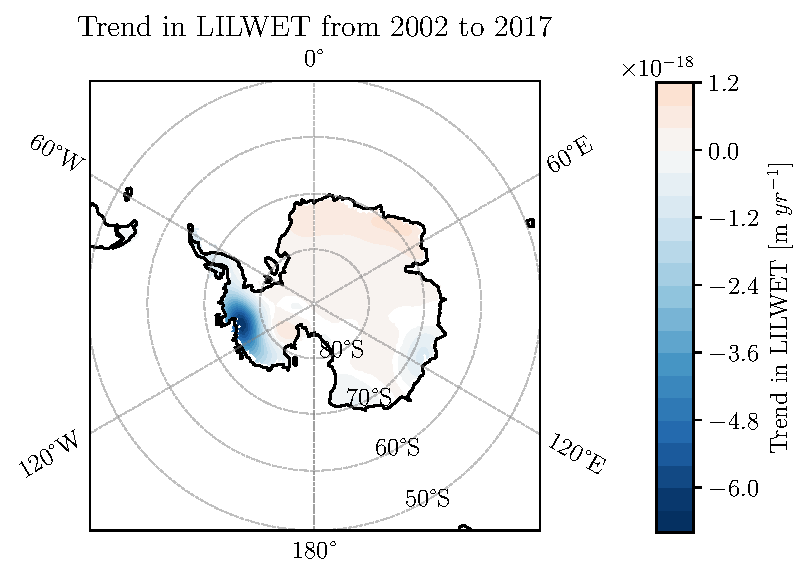
\includegraphics{images/2021w5/chapter7/hres/trend_spatial_LIC}
    \caption{Trend in Antarctic \gls{lilwet} from 2002 to 2007. Only statistically significant trends have been plotted, i.e. with a p-value $\leq$ 0.05.}
    \label{fig:lilwet_trend}
\end{figure}

Looking at figure \ref{fig:lilwet_trend} we can gain some understanding of how \gls{lilwet} changed from 2002 to 2007. This tells a similar story to what we saw in figure \ref{fig:lilwet_mean}, in that the \gls{wais} exhibits a large and significant decrease over time period. It is worth noting that while the trends over the rest of the continent and the \gls{eais} are small they are still statistically significant (with a p-value $\leq$ 0.05). This means that while we are mostly motivated to understand the strong decrease in the \gls{wais}, we cannot fully ignore the behaviour of ice in the \gls{eais}. Our final step before investigating the different variables which could impact the behaviour of Antarctic \gls{lilwet} is to look at the timeseries of mean Antarctic \gls{lilwet} from 2002 to 2017 (see Figure \ref{fig:lilwet_timeseries}).

\begin{figure}[!hbt]
    \centering
    \includegraphics{}
    \caption{Time series of mean Antarctic \gls{lilwet} from 2002 to 2007.}
    \label{fig:lilwet_timeseries}
\end{figure}

\textcolor{red}{Plot of mean time-series of Antarctic ice}

The simplest thing we can do at this point is to compare the mean time series of this with different variables.

\section{Comparing land ice with different variables}
For the first step in analysis here we plotted the mean values for both land ice and other environmental variables, considering only the grid points where we have data for land ice.

\subsection{Trends in different variables}
\textcolor{red}{Plot of trend in Temperature, subsurface temperature, ozone, precipitation, wind speed}
\begin{figure}[!hbt]
    \centering
    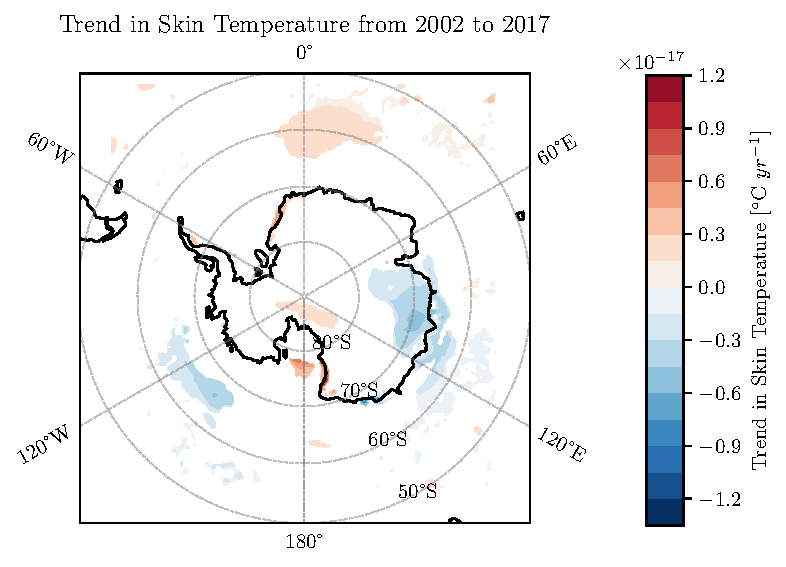
\includegraphics{images/2021w5/chapter7/hres/trend_spatial_skt}
    \caption{Trend in skin temperature over Antarctica from 2002 to 2017}
    \label{fig:trend_skt_02_17}
\end{figure}
\begin{figure}[!hbt]
    \begin{subfigure}[b]{0.5\textwidth}
    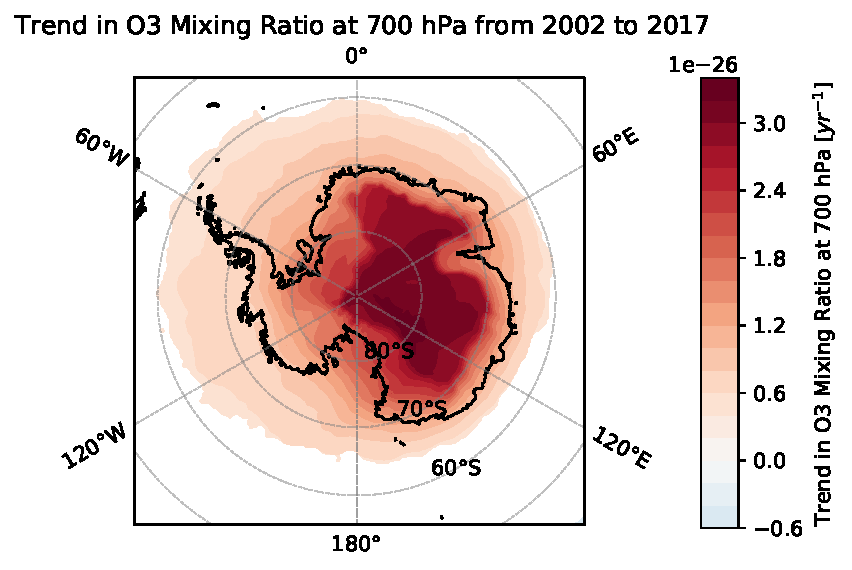
\includegraphics[width=\textwidth]{images/2021w5/chapter7/hres/trend_spatial_o3_700}
    \end{subfigure}
    \begin{subfigure}[b]{0.5\textwidth}
    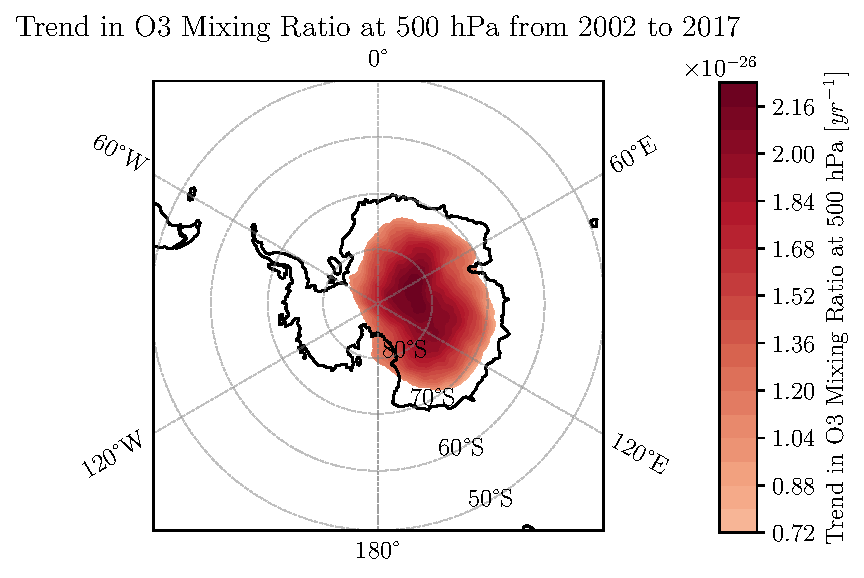
\includegraphics[width=\textwidth]{images/2021w5/chapter7/hres/trend_spatial_o3_500}
    \end{subfigure}
    \begin{subfigure}[b]{0.5\textwidth}
    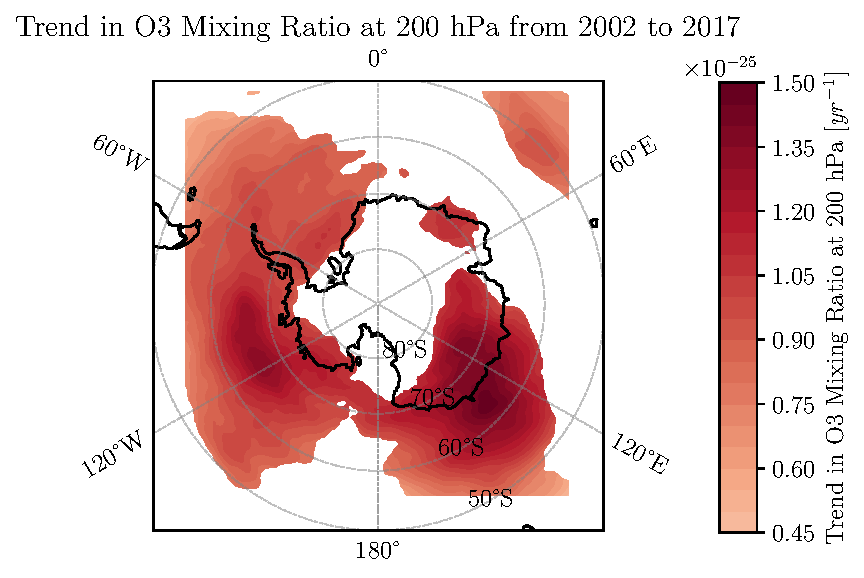
\includegraphics[width=\textwidth]{images/2021w5/chapter7/hres/trend_spatial_o3_200}
    \end{subfigure}
    \begin{subfigure}[b]{0.5\textwidth}
    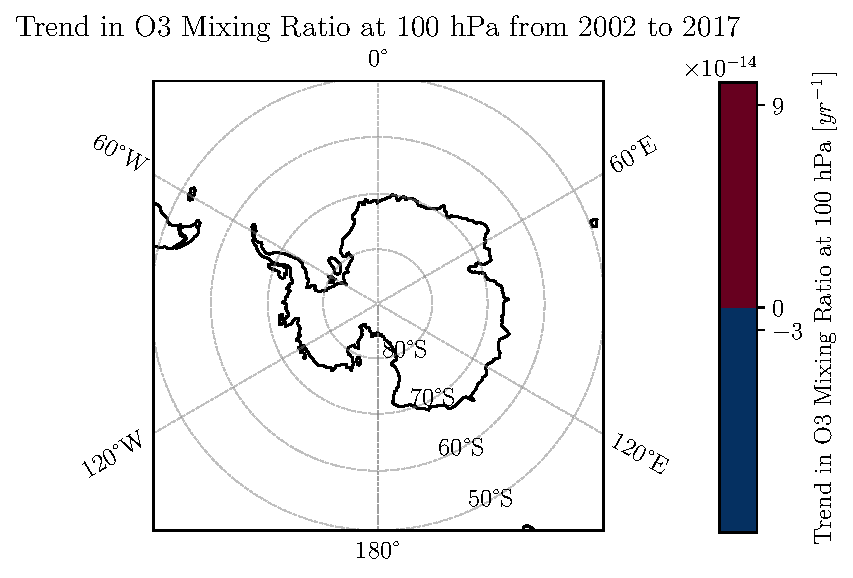
\includegraphics[width=\textwidth]{images/2021w5/chapter7/hres/trend_spatial_o3_100}
    \end{subfigure}
    \begin{subfigure}[b]{0.5\textwidth}
    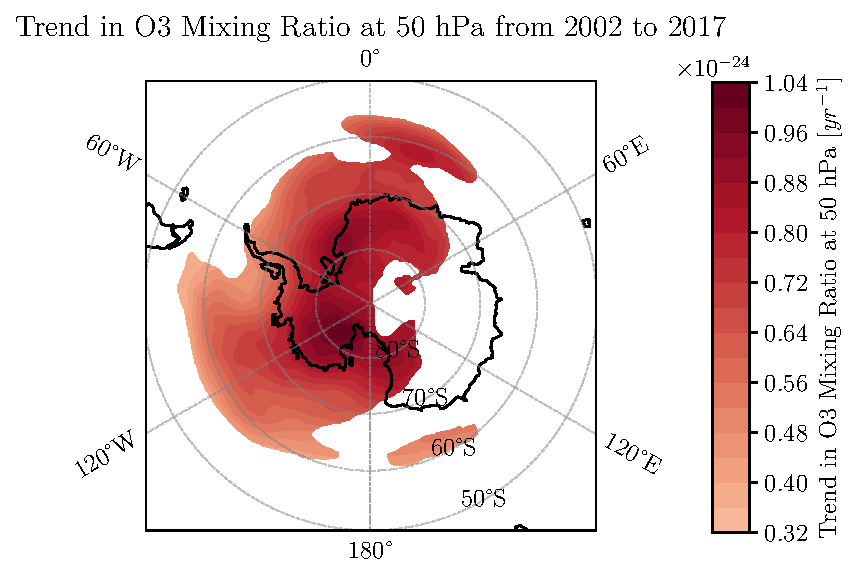
\includegraphics[width=\textwidth]{images/2021w5/chapter7/hres/trend_spatial_o3_50}
    \end{subfigure}
    \caption{Trend in skin temperature over Antarctica from 2002 to 2017 \textcolor{red}{make these sub-figures in python}}
    \label{fig:trend_skt_02_17}
\end{figure}
\begin{figure}[!hbt]
    \centering
    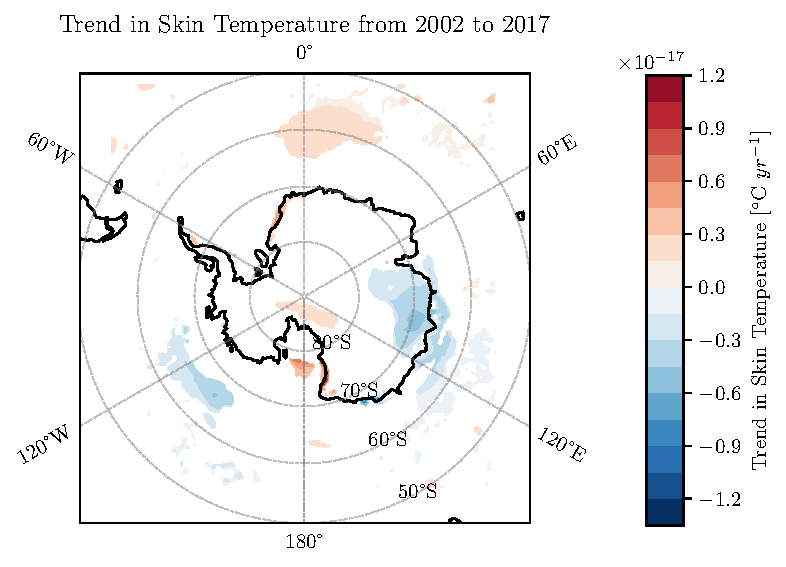
\includegraphics{images/2021w5/chapter7/hres/trend_spatial_skt}
    \caption{Trend in skin temperature over Antarctica from 2002 to 2017}
    \label{fig:trend_skt_02_17}
\end{figure}
\begin{figure}[!hbt]
    \centering
    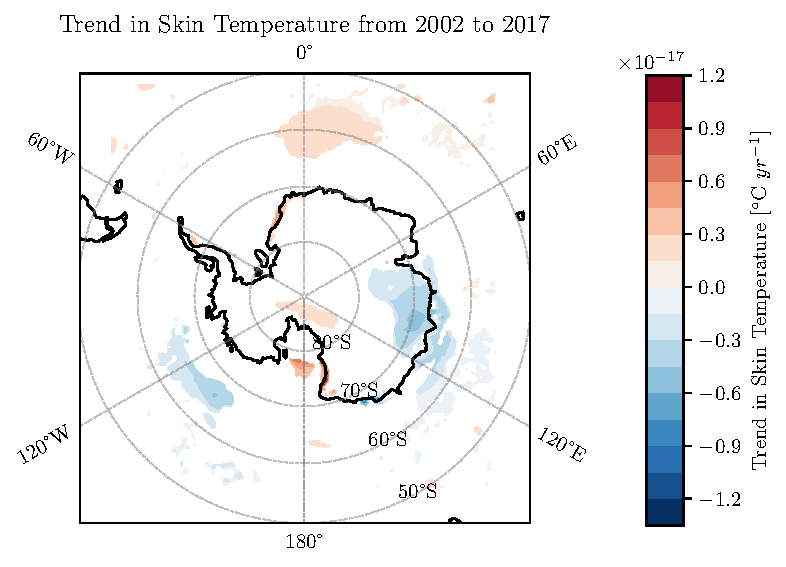
\includegraphics{images/2021w5/chapter7/hres/trend_spatial_skt}
    \caption{Trend in skin temperature over Antarctica from 2002 to 2017}
    \label{fig:trend_skt_02_17}
\end{figure}
\begin{figure}[!hbt]
    \centering
    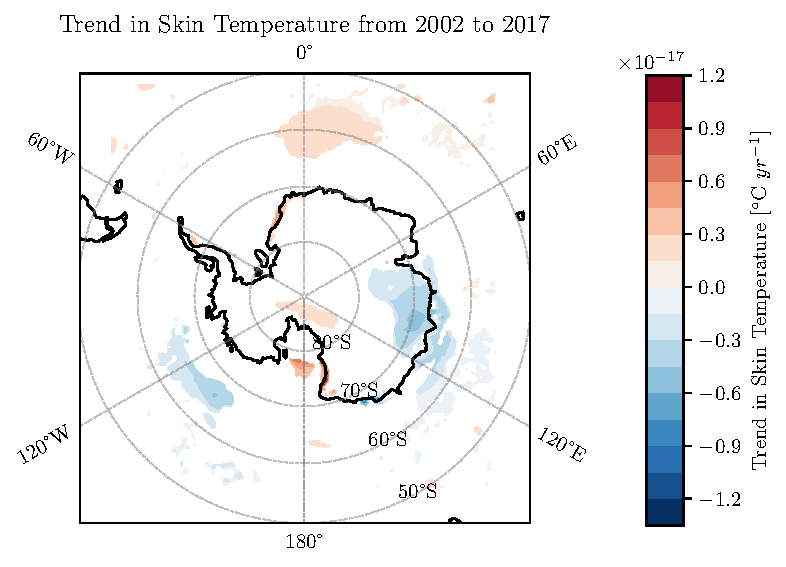
\includegraphics{images/2021w5/chapter7/hres/trend_spatial_skt}
    \caption{Trend in skin temperature over Antarctica from 2002 to 2017}
    \label{fig:trend_skt_02_17}
\end{figure}
\begin{figure}[!hbt]
    \centering
    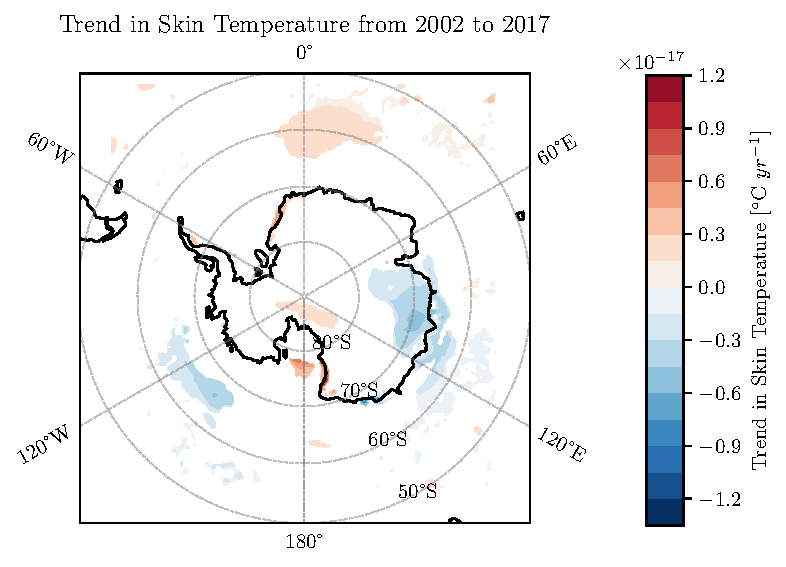
\includegraphics{images/2021w5/chapter7/hres/trend_spatial_skt}
    \caption{Trend in skin temperature over Antarctica from 2002 to 2017}
    \label{fig:trend_skt_02_17}
\end{figure}

\subsection{Visual time series comparison}

\subsection{Co-spatial Correlations}

\section{Identifying drivers for significant decrease}

\subsection{Identifying region with significant decrease}

\subsection{Spatial correlations}

\subsection{Regressions}

\section{Discussion and implications of these results}

\end{document}